\documentclass[11pt, spanish]{article}
\pagestyle{empty}

%acentos de la forma � en vez de \'a
\usepackage[spanish]{babel}
\usepackage[utf8]{inputenc}

%Enumeración con columnas que se usa con \begin{multicols}{2} \begin{enumerate}
\usepackage{multicol}
\usepackage{multirow}


%Para poder usar begin comment
\usepackage{verbatim}

%Teoremas
\usepackage{amsthm}
\theoremstyle{plain}
\newtheorem{teo}{Teorema}


%letras para enumerar
\makeatletter\renewcommand\theenumi{\@alph\c@enumi}\makeatother\renewcommand\labelenumi{\theenumi)}

%m�rgenes
\usepackage[left=2cm,top=2cm,right=2cm]{geometry}

\usepackage{fancyhdr}
\pagestyle{fancy}
\usepackage{enumerate}

%conjuntos N, Q, R, Z, C
\usepackage{dsfont}
\newcommand{\N}{\mathds{N}}
\newcommand{\Q}{\mathds{Q}}
\newcommand{\R}{\mathds{R}}
\newcommand{\Z}{\mathds{Z}}
\newcommand{\C}{\mathds{C}}
\newcommand{\M}{\mathcal{M}}
\newcommand{\Pol}{\mathcal{P}}

%Transformada de Laplace
\renewcommand{\L}{\mathcal{L}}

%Probabilidades
\newcommand{\PP}{\mathbb{P}}
\newcommand{\E}{\mathbb{E}}
\newcommand{\B}{\mathcal{B}}
\newcommand{\Var}{\mathbb{V}\text{ar}}

%l�gica
\newcommand{\ssi}{\Leftrightarrow}

%funciones
\newcommand{\function}[5]{  \begin{array}{rl}
                                #1: #2 &\longrightarrow #3 \\
                                #4 & \longmapsto #1\left(#4\right)= #5
                            \end{array} }

\newcommand{\funcion}[3]{#1: #2 \longrightarrow #3 }
\newcommand{\parteentera}[1]{[#1]}

%%%operadores matematicos
\usepackage{mathtools}
\DeclarePairedDelimiter\abs{\lvert}{\rvert}%
\DeclarePairedDelimiter\norm{\lVert}{\rVert}%
\newcommand{\tr}{\text{tr}}


% Swap the definition of \abs* and \norm*, so that \abs
% and \norm resizes the size of the brackets, and the 
% starred version does not.
\makeatletter
\let\oldabs\abs
\def\abs{\@ifstar{\oldabs}{\oldabs*}}
%
\let\oldnorm\norm
\def\norm{\@ifstar{\oldnorm}{\oldnorm*}}
\makeatother
% % % % % % % % % %
%\providecommand{\abs}[1]{\lvert#1 \rvert}
%\providecommand{\norm}[1]{\lVert#1 \rVert}
%\providecommand{\pin}[2]{\left< #1,#2 \right>} %producto interno

\providecommand{\dpartial}[2]{\frac{\partial #1}{\partial #2}} %derivada parcial

\usepackage{amssymb}
\usepackage{amsmath, amsthm, amsfonts}

%Im�genes
\usepackage{graphicx}
\usepackage{float}
\begin{document}
\fancyhead[L]{Facultad de Ciencias Físicas y Matemáticas}
\fancyhead[R]{Universidad de Chile}

\begin{flushleft}
  \textbf{IN6228-1 Teoría de Juegos 2018}
  \\\textbf{Profesor:} José Correa.
  \\\textbf{Auxiliares:} Carlos Bonet y Andrés Cristi.
\end{flushleft}


\begin{center}
  \large{\textbf{Clase Auxiliar 2\\ 11 de Abril de 2018}}
\end{center}

%\begin{flushleft}



\begin{itemize}
\item[\textbf{P1.}] Considere el siguiente juego de 2 jugadores. El jugador 1 elige un número $x_1\in [1,10]$. Luego el jugador 2 elige un número entre $x_1+1$ y $x_1+10$. El jugador 1 observa este número y elige un número $x_2$ entre $y_1+1$ e $y_1+10$ y así sucesivamente, en cada turno uno de los jugadores adiciona una catidad en $[1,10]$. El ganador es el primero que declara el número 100, quien recibe $\$ 100$ y el perdedor no recibe nada. Encuentre el EPS de este juego. ¿Quién gana?

\item[\textbf{P2.}] Probaremos en este problema la siguiente versión del teorema de existencia de equilibrio que es levemente más fuerte.
\begin{teo}
Consideremos un juego con espacios de estrategias $S_i\subseteq \R^{d_i}$
convexos compactos y funciones de pago $u_i:\prod_{i=1}^n \rightarrow \R$ continuas y tales que $x_i\mapsto u_i(x_i,s_{-i})$ es cuasicóncava, es decir los conjuntos de nivel $\{ x_i\in S_i: u_i(x_i,s_{-i})\geq \lambda\}$ son convexos. Entonces existe un equilibrio de Nash.
\end{teo}
Para ello
\begin{enumerate}
    \item Considere una función $M:C\rightarrow 2^C$, con $C$ convexo compacto, $M(x)$ convexo cerrado y no vacío para todo $x\in C$. Suponga que además para todo$x\in C$ y $\varepsilon>0$ existe $\delta>0$ tal que
    \[
    \norm{ x'-x}<\delta \Rightarrow M(x')\subseteq M(x) + B(0,\varepsilon).
    \]
    Pruebe que existe una función $\Phi:C\rightarrow C$ continua tal que $d((x,\Phi(x)),M)\leq \varepsilon$ para todo $x\in C$.
    \item Pruebe que $M$ tiene un punto fijo, es decir, $x^* \in M(x^*)$.
    \item Concluya el teorema.
\end{enumerate}

\item[\textbf{P3.}] Considere el juego con 3 jugadores siguiente con pagos dados por la figura, donde el jugador 1 elige una fila, el jugador 2 elige una columna y el tercero elige una de las 3 tablas.
\begin{figure}[h!]
    \centering
    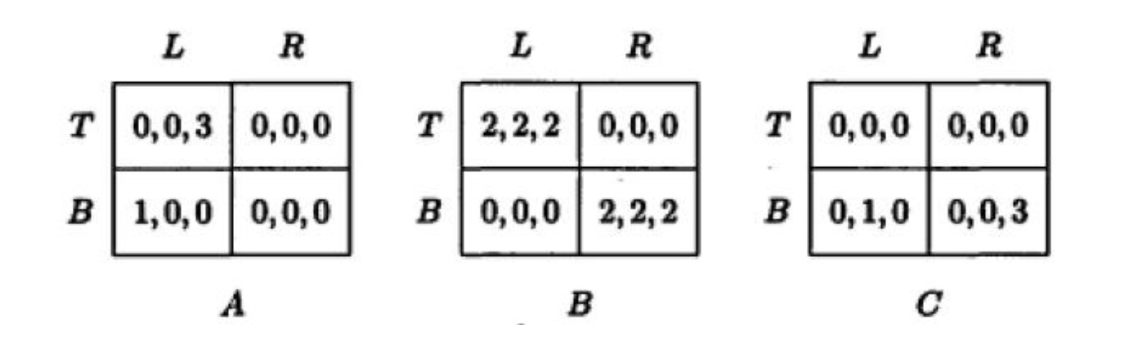
\includegraphics[scale=0.4]{Tablas.png}
    \label{fig:my_label}
\end{figure}
\begin{enumerate}
    \item Encuentre equilibrios en estrategias puras con pagos $(1,0,0), (0,1,0)$ y $(0,0,0)$.
    \item Encuentre un equilibrio correlacionado donde los jugadores 1 y 2 juegan $(T,L)$ y $(B,R)$ con igual probabilidad.
    \item Suponga que el jugador 3 no es estratégico y siempre juega $B$, por lo que en el juego participan solamente los jugadores 1 y 2. Encuentre todos los equilibrios de Nash (puros y mixtos).
\end{enumerate}



\end{itemize}
\end{document} 
